\todo{Purpose of the chapter
 Structure of the chapter
 Central themes of the chapter}

\section{Non-functional requirements} {
\label{sec:non_functiona_requirements}

	The following non-functional requirements are considered key to the success of this project:

	\begin{description}
		\item[Modularity:] The project should be highly modular, so parts of the system can be reused and easily integrated into the group project.
		\item[Performance:] The response time of the system is a major concern when working with a large dataset. The time to load the visualisation is highly dependent on the size of the dataset, graphical processing, network bandwidth and latency. However, once the visualisation has loaded, the user should be faced with near immediate response times (\textless 1 second).
		\item[Scalability:] This is important when modifying the size of the dataset used with a visualisation. The visualisation should be capable of handling increased processing with a larger dataset. Not only this, but the information should remain mapped to the correct locations in the scene with increased volumes of data.
		\item[Testability:] Highly testable code is important when writing test suites, so all aspects of the system can be easily tested to locate faults. In JavaScript:
			\begin{itemize}
				\item A common technique is to hide variables through the use of closure, which leads to untestable code. These variables should be replaced with public variables that are prefixed with an underscore, to indicate they are not a part of the public API.
				\item Promises should not be used within a constructor.
				\item Anonymous functions should be replaced with named functions so they can be tested.
				\item Dependency injection should be used through RequireJS, so all dependencies can be mocked.
			\end{itemize}
	\end{description}

}

\section{Methodology} {
\label{sec:methodology}

	A rapid application development (RAD) approach was undertaken when developing this project. This methodology focuses on iterative development and the rapid construction of prototypes, instead of investing significant amounts of time into planning. RAD enables the software to be written quickly through the reuse of software components and engaging in less formal reviews. This process also performs unit, integration and system testing at the end of each construction phase.

	\todo{insert diagram}

	In this project, each visualisation can be thought of as a single prototype, where parts of the first prototype can be reused for the second visualisation. Testing should be performed during the course of the project, but particularly when a major component of a prototype has been developed, such as data filtering.

	\todo{iterative, agile}

	% An agile methodology will be used throughout the project, as it promotes iterative development, adaptive planning, early prototyping, and encourages flexible and rapid response to changing requirements. This is in contrast to the more traditional methodology, waterfall, which implies a much more rigid workflow, where all requirements are set in stone early in the project. The agile approach gives the project more flexibility, which is required for a project of greater complexity.
	
	% \subsection{Scrum} {

	% 	Scrum is an iterative and incremental agile methodology, in consists of short iterative `sprints' of focused development. The decided sprint length of this project 2 weeks, and conveniently corresponds with the fortnightly client meetings.
		
	% 	Before each sprint, tasks are created and prioritised. These tasks are then assigned evenly across team leaders, and then are further distributed to their team members. This process can take a day or so after the last sprint has finished, using the client's feedback as motivation as to what to include in the sprint. A sprint is then started, and development is generally 'locked' until the completion of the sprint. This keeps teams focused on the issues for the sprint, which have been decided to be the most important.
		
	% 	The chosen issue tracking tool, JIRA, wholly supports the scrum methodology, with in-built features for creating sprints, epics and user stories. This in-built tooling support, combined with its iterative development cycle, makes Scrum a convenient and appropriate methodology for the project.
		
}

\section{Dataset} {
\label{sec:dataset}

	% \todo{convert to past tense and make datasets solid}

	% As discussed in Section~\ref{sec:deliverables}, the visualisations began with generated data so development could begin immediately. Using generated data brings control over the size of the dataset applied to a prototype and enables the scalability of each visualisation can be tested. 

	% Following the use of fake data, each prototype had real datasets applied to them. By using the same data for both prototypes, their differences in computational requirements and scalability could be compared and analysed. GeoNames~\footnote{\bibentry{wick2005geonames}} is a geographical database that stores population data for a significant number of cities and their respective latitude and longitude coordinates. This database falls under a creative commons attribution license and will be used for both visualisations because there are no copyright concerns or immediate issues when reading and parsing the data it provides. However, some unnecessary information contained in a GeoNames dataset (such as \emph{geonameid}, \emph{feature class} and  \emph{dem}) will need to be removed. The format of the data should also be modified (from a tab separated list to a JavaScript array) when used with a prototype. These steps are necessary so the visualisations can read the data efficiently and hence reduce the loading time for the user. Other datasets can be obtained from Earthdata~\footnote{\bibentry{nasa2000data}}, but will require further investigation regarding how to extract the information from the available databases.

	% Once real data has been applied to both prototypes, the visualisations will be integrated into a live system for the teaching analytics component of the final year project. The amount of touch gestures that particular system components receive and the progress made by students, groups and tutorials will need to be collected and stored in the database. This data can be visualised to aid teachers in analysing ongoing student progress.

	\subsection{Structure} {
	\label{sec:dataset_structure}

		\todo{mention flat vs metadata, performance issues}

		The data for the visualisations can easily be represented as a flat array and may need to be preprocessed, which depends on the format of the data. This data representation has also been adopted by The WebGL Globe Chrome Experiment~\footnote{\bibentry{google2011globe}}, as shown in Appendix~\ref{app:globe}, is a great example of visualising a large dataset in an efficient way. This open platform project clearly demonstrates that the goals of this project are achievable. They encourage users to use their own datasets, ensuring a certain level of scalability and applications with geographical data.

	}

}

\section{User interface} {
\label{sec:user_interface}

	The user interface for this system has combined Google's Material Design with 3D elements, to simplify the way users interact with the system.

	\subsection{Material Design} {
	\label{sec:material_design}

		Material Design is a visual language developed by Google that synthesises classic design principles with current technologies. This design revolves around three principles which have been defined in Figure~\ref{fig:material_design_principles}.

		\newcommand{\materialwidth}{0.328\textwidth}
\begin{figure}[H]
	\centering
	\begin{subfigure}[b]{\materialwidth}
		
\includegraphics[width=\textwidth]{images/design/material/metaphor}
		\caption{Material is the metaphor}
		\label{fig:material_design_metaphor}
	\end{subfigure}
	\begin{subfigure}[b]{\materialwidth}
		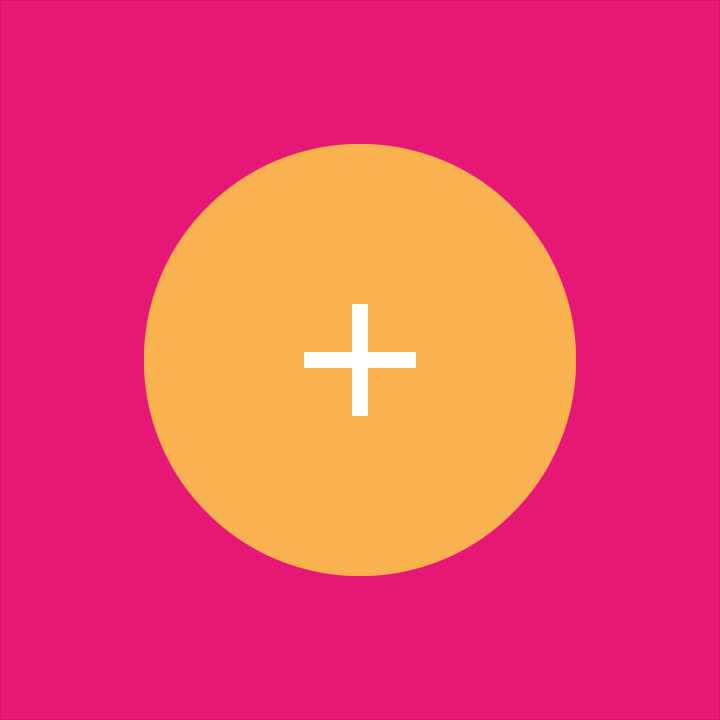
\includegraphics[width=\textwidth]{images/design/material/bold}
		\caption{Bold, graphic, intentional}
		\label{fig:material_design_bold}
	\end{subfigure}
	\begin{subfigure}[b]{\materialwidth}
		
\includegraphics[width=\textwidth]{images/design/material/motion}
		\caption{Motion provides meaning}
		\label{fig:material_design_motion}
	\end{subfigure}
	\caption[Material Design principles]{Material Design principles.}
	\label{fig:material_design_principles}
\end{figure}


		Material Design uses the fundamentals of light, surface and movement to convey how objects move, interact and exist in space and in relation to each other. Elements such as typography, grids, space and colour have been designed to create meaning, maintain user focus and establish a hierarchy using depth effects. These principles aim to provide users with a unified, immersive experience across platforms and device sizes, by focusing on user actions and retaining continuity between transitions~\footnote{\bibentry{google2015material}}.

		Material Design composes the specifications for many components

		\todo{material design to match FYP and modern look and feel}

	}

	\subsection{3D elements} {

		The 3D elements encompass the visualisation

	}

	\subsection{Layout} {

		A mockup of the user interface has been shown in Figure~\ref{fig:user_interface_mockup}.

		\begin{figure}[H]
	\centering
    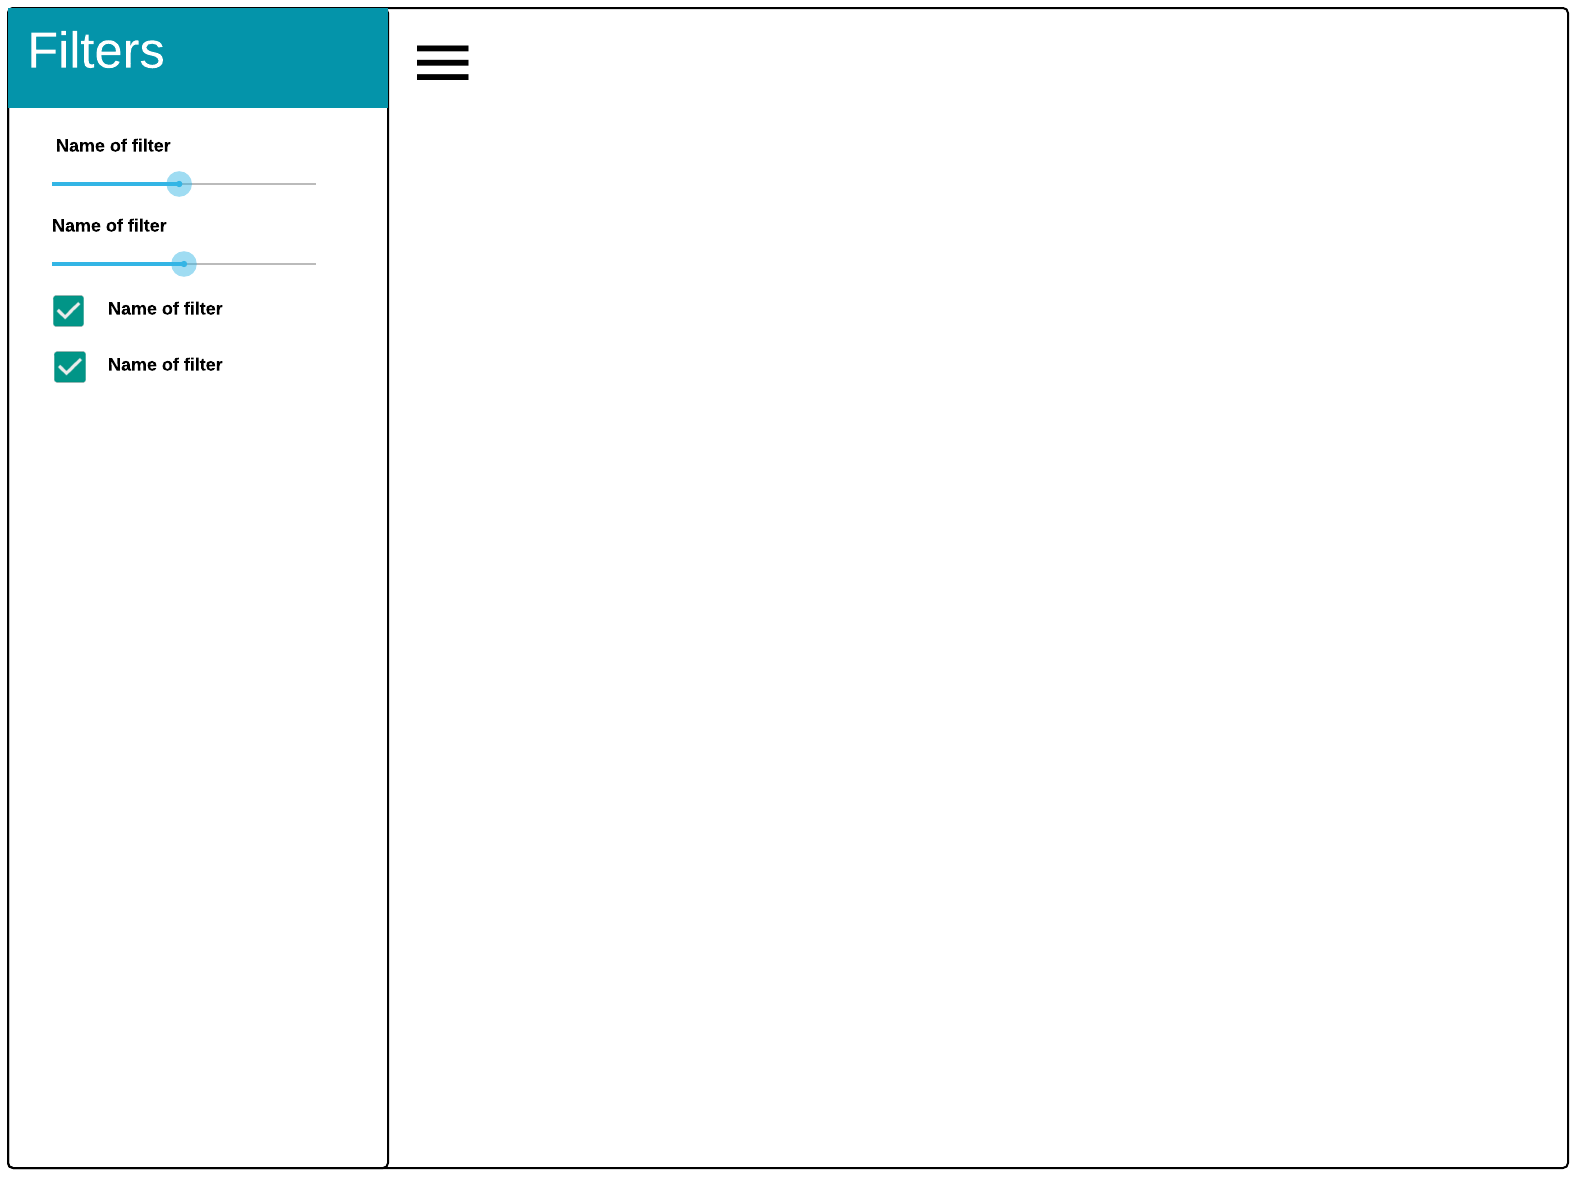
\includegraphics[width=\textwidth]{images/design/interface}
    \caption[User interface mockup]{User interface mockup.}
    \label{fig:user_interface_mockup}
\end{figure}


		This design incorporates two sections, the sidebar / classic drawer navigation and the scene. The sidebar is available for users to filter data.

	}

}

\section{Architecture} {
\label{sec:architecture}
	
	\todo{three-tier: presentation, logic, data

		inheritance

		design patterns

		architecture diagram}

}
